%\section{Vāju radioastronomisko objektu novērojumu programmrisinājumu}
\section{MPI integrācija kalibrācijas procesā}

Balstoties uz to, ka jēldatu apstrādes process ir laikietilpīgs, kā arī resursietilpīgs process, to ir nepieciešams efektīvi paralelizēt. Veids, kā tas tiek darīts Bakalaura darba datu apstrādes sistēmā, ir, izmantojot \textit{Python} bibliotēkas \textit{mpi4py} \cite{mpi-docs} iespējas, kura realizē \textit{Message Passing Interface} jeb \textit{MPI} protokolu python valodā, kas atļauj \textit{Python} procesam izmantot vairākus kodolus vienlaicīgi.

Lai testētu \textit{MPI} integrāciju kalibrācijas procesā, tika izveidots programrisinājums, kurš paredzēts izmantošanai ar deviņiem \textit{MPI} procesiem, kur process nr. 1  atbild par failu apstrādes organizēšanu un masīvu apstrādi, bet procesi 2-9 veic jēldatu nolasīšanu, kura aprakstīta nodaļā \ref{read-data} Izpildes procesa piemērs attēlots pielikumā \ref{appendix:old-version}, kur pa soļiem attēlota datu apstrādes loģika un informācijas plūsma. Procesi attēloti, kā apļi, kuru centrā norādīts fails, kurš patreiz tiek apstrādāts.

%Process 0 sākotnēji nolasa visus jēldatus direktorijā, tad katrus 8 failus sūta savam procesam. Šie procesi nolasa datus un rezultējošo masīvu atsūta atpakaļ procesam 0, kas uzsāk kalibrācijas procesu. Kad kalibrācija ir pabeigta un jaunais rezultāts ir saglabāts, process cikliski atsākas nākamajiem 8 failiem, līdz apstrādāti visi dati. Kad visi dati nolasīti, process 0 nosūta pārējiem procesiem informāciju par datu apstrādes beigām un šie procesi pārstāj darbību.

Ņemot vērtā to, ka sākotnējā MPI algoritma versija bija spējīga izmantot tikai 9 procesus datu apstrādei, bet pieejami bija daudz vairāk skaitļošanas resursu, algoritms tika pilnībā pārveidots. Algoritma versija Bakalaura nodošanas laikā spējīga datus apstrādāt neierobežotā kodolu skaitā, pilnvērtīgi izmantojot visus iedalītos kodolus.

Algoritma process nr. 1 uzlabotajā algoritmā atbild par kalibrēšanu un datu apvienošanu. Process nr. 2 - par pārējo procesu pārvaldību un failu nosaukumu nodošanu pārējiem procesiem. Procesam ar numuru 3 ir iedalīts speciāls uzdevums - nokalibrēt dat failus, jo dat failu apstrādes process ir ļoti ātrs un lietotāja ērtības dēļ, visas darbības tiek koncentrētas vienotā algoritmā. Kad process nr. 3 ir nokalibrējis dat failus, tas tiek pievienots pārējiem, jēldatu nolasīšanai paredzētajiem, procesiem. Tas nozīmē, ka algoritmu ir nepieciešams startēt, izmantojot vismaz 3 procesus, lai gan algoritms paredzēts daudz vairāku procesu izmantošanai. Izpildes procesa piemērs attēlots pielikumā \ref{appendix:new-version}, kur attēlota procesu komunikācija un datu apstrādes process. Kā piemērs, tiek apskatīts potenciālā komunikācija starp astoņiem procesiem, taču līdzīgs rezultāts ir iegūstams jebkurā procesu daudzumā. Jāņem vērā, ka katrā algoritma izpildes reizē komunikācija var atšķirties, jo nolasīšanas ātrums nav konstants. Procesi pielikumā \ref{appendix:new-version} attēloti kā apļi, kuru centrā norādīts procesa pieejamības stāvoklis.

Process nr. 2 ir algoritma sarežģītākā daļa, jo ir nepieciešams nodrošināt, ka visiem iedalītajiem procesiem vienmēr ir iedalīts savs fails un iedalītais process strādā pie faila nolasīšanas, kā arī jānodrošina, ka visi dati ir apstrādāti. Tas tiek realizēts ar masīvu, kur katrs elements atbilst procesa statusam. Sākotnēji procesu vērtības inicializētas ar vērtību 1, izņemot pirmās 3, jo minētie procesi jau ir aizņemti.
Tad process, ciklā visu failu sarakstam, sūta failu ceļu pirmajam procesam, kurš ieņēmis stāvokli "1". Ja faila ceļš nosūtīts, atbilstošais procesa statuss attiecīgi ir mainīts uz 0, lai attēlotu, ka tas ir aizņemts. Ja visi procesi ir aizņemti, process 2 gaida uz kādu no pārējiem procesiem, lai tas nosūtītu apstiprinošu ziņu, ka dati nolasīti un iedala attiecīgajam procesam jaunu failu apstrādei. Kad visi faili nolasīti, pārējiem procesiem tiek aizsūtīta ziņa par datu apstrādes beigām un procesi apkopo savus datus vienā datu struktūrā, kuru nosūta procesam 1 tālākai apstrādei.  

Algoritmam tika veikti veiktspējas testi, kuri aprakstīti \ref{algorithm-eval} nodaļā. Tiek apskatītas atšķirības no vecā algoritma versijas veiktspējas, kā arī fināla versijas algoritma veiktspējas atkarība no kodolu daudzuma.




%\section{Stoka parametri (Varbūt neizmantos)}
%Lai nodrošinātu datu integritāti, tika apskatīti arī datu Stoka parametri - vērtību kopa, kas apraksta polarizācijas radiācijas stāvokli. Balstoties uz rakstu par Nançay radioastronomijas observatorijas iegūtajiem rezultātiem no 2007-2009 gada \cite{nancay}, kurā tika aprakstīta informācija par laika periodā novērotajām maiņzvaigznēm, bija iespējams salīdzināt šos rezultātus ar bakalaura darba laikā apskatītā objekta rezultātiem. 


%Bakalaura darba ietvaros, tika izpētīts \textit{The Measurement of Polarization in Radio Astronomy} \cite{stokes} raksts, lai iegūtu formulas cirkulārās polarizācijas Stokes parametru aprēķinam:
%\begin{equation}
%I= \langle E_R^2 \rangle + \langle E_L^2 \rangle \tag{2.2.5.1}\label{eq:2.2.5.1}
%\end{equation}
%\begin{equation}
%Q = 2 \langle Re(E_R E_L^*) \rangle = 2 \langle E_R E_L \cos{\delta_{RL}} \rangle \tag{2.2.5.3}\label{eq:2.2.5.3}
%\end{equation}
%\begin{equation}
%U = 2 \langle Im(E_R E_L^*) \rangle = 2 \langle E_R E_L \sin{\delta_{RL}} \rangle \tag{2.2.5.4}\label{eq:2.2.5.4}
%\end{equation}
%\begin{equation}
%V= \langle E_R^2 \rangle - \langle E_L^2 \rangle \tag{2.2.5.5}\label{eq:2.2.5.5} 
%\end{equation}

%\textbf{paskaidrojums un kur/kāpēc tiek izmantots}
%kur: 
%\begin{tabbing}
%\phantom{\hspace{10mm}}\= \kill
%$I$\>                   =$I$\\
%$Q$\>                   = $Q$\\
%$U$\>                   = $U$\\
%$V$\>                   = $V$\\
%$E_R^2$\>               = $E_R^2$\\
%$E_L^2$\>               = $E_L^2$\\
%$\delta_{RL}$\>         = $\delta_{RL}$\\

%\end{tabbing}



%Rakstā tika apskatītas kopā 70 zvaigznes, taču bakalaura darba ietvaros, tika apskatīta tikai informācija par RLMI maiņzvaigni, jo minētais objekts tika novērots, kā komētu kalibrators. 



\section{Anomāliju detektācija} \label{anomalies}
Veicot novērojumus, pastāv risks, ka konkrēts skans ir ticis bojāts kādu inženiertehnisku problēmu dēļ un nav izmantojams datu apstrādē. Lai realizētu veiksmīgu datu apstrādes procesu, bojātos kalibrācijas rezultātus ir nepieciešams identificēt.  
Gadījumos, kur novērojuma skans ir bojāts, rezultējošā spektra vērtības ieņem vērtības, kas ir daudz lielākas, par pareizu skanu rezultātiem. Augstās amplitūdas vērtības tiek iegūtas augstas sistēmas temperatūras vērtības rezultātā, tāpēc identificējot pēkšņas augstas sistēmas temperatūras vērtības, ir iespējams atrast bojātos skanus ar pietiekami augstu precizitāti, lai pārējo skanu kopas rezultāts būtu izmantojams.

Bakalaura darba ietvaros, datu anomālijas tiek detektētas, izmantojot standarta vērtību jeb \textit{z-score}. \textit{Z-score} ir statistikas rādītājs, kas norāda vērtības attiecību pret vidējo. Kā vidējā vērtība, šajā gadījumā tiek uzskatīta izslēgtas trokšņa diodes sistēmas temperatūras vidējā vērtība pēc formulas:

\begin{equation}
\overline{Tsys} = \frac{\overline{T_{sys,sig}^{off,left}} + \overline{T_{sys,sig}^{off,right}} + \overline{T_{sys,ref}^{off,left}} +  \overline{T_{sys,ref}^{off,right}} }{4} \tag{1.7.1}\label{eq:1.7.1} 
\end{equation}
kur: 
\begin{tabbing}
\phantom{\hspace{20mm}}\= \kill
$\overline{T_{sys,sig}^{off,left}}$\> = Lokālā oscilatora sistēmas temperatūra ar izslēgtu trokšņa diodi kreisajai \\ cirkulārai polarizācijai\\
$\overline{T_{sys,sig}^{off,right}}$\> = Lokālā oscilatora sistēmas temperatūra ar izslēgtu trokšņa diodi labajai \\ cirkulārai polarizācijai\\
$\overline{T_{sys,ref}^{off,left}}$\>   = References lokālā oscilatora sistēmas temperatūra ar izslēgtu trokšņa diodi \\ kreisajai cirkulārai polarizācijai\\
$\overline{T_{sys,ref}^{off,right}}$\>   = References lokālā oscilatora sistēmas temperatūra ar izslēgtu trokšņa diodi \\labajai cirkulārai polarizācijai\\
\end{tabbing}

Lai iegūtu precīzākus rezultātus, iespējams izmantot katras sistēmas temperatūras spektra vidējo vērtību, kopumā rēķinot \textit{z-score} katram sistēmas temperatūras masīvam, taču, pēc noklusējuma tiek izmantots vidējā izslēgtas trokšņa diodes sistēmas temperatūra, jo otra metode nav pietiekami daudz analizēta, lai sniegtu pārliecinošus rezultātus.

Izmantojot vidējo vērtību un \textit{scipy stats} piedāvāto funkciju z-score aprēķināšanai, tiek atlasītas visas vērtības, kur standarta vērtība ir lielāka par 2 jeb divas standartnovirzes lielāka par vidējo vērtību. Detektētās anomālijas tiek ierakstītas kalibrācijas log failā, kopā ar skana numuru un skana ierakstīšanas laiku turpmākai analīzei, lai palīdzētu identificēt potenciālos problēmu cēloņus nākotnē.

Sākotnējais anomāliju detektēšanas algoritms izmantoja individuālā spektra vidējo vērtību, kuru salīdzināja ar visu novērojumu vidējo vērtību. Lai gan šī metode detektēja spēcīgi bojātos skanus, bija problēmas ar iegūto rezultātu precizitāti. Dažkārt algoritms klasificēja nebojātos datus kā bojātus, kas samazināja rezultātu integritāti, līdz ar to bija nepieciešams atrast alternatīvu, šajā gadījumā, z-score, kurš, lai gan strādā uz līdzīga principa, bija spējīgs iegūt precīzākus rezultātus.

Tika izvirzīta hipotēze, kurā bojāto skanu ignorēšanas vietā, varētu prognozēt sistēmas temperatūru konkrētajā skanā un aizvietot bojāto rezultātu ar pareģoto. Pareģot temperatūru ir iespējams ļoti daudzos veidos, taču Bakalaura darba ietvaros tika apskatītas divas metodes - vismazāko kvadrātu polinoma pielāgošana jeb \textit{polyfit} un veivletu pielietošana spektra formas iegūšanai.

Izmantojot \textit{polyfit} funkciju, tika pareģota taisne, kura izmanto pirmo piecu un pēdējo piecu skanu vidējās vērtības. Šāda veida prognozēšana ir bīstama, jo ir iespējams, ka bojātais skans būs kādā no minētajām 10 vērtībām, līdz ar to, pareģotais rezultāts būs bojāts. Lai gan varētu vairāk modificēt minēto metodi, balstoties uz pieredzi citos novērojumos, tika izteikts priekšlikums izmantot veivletus. 

Izmantojot zemas precizitātes slieksni veivletu transformācijā, tiek iegūts spektrs, kas vāji atbilst sākotnējam spektra vērtībām, taču saglabā sākotnējo spektra formu. Līdz ar to, skanos, kur tiek detektēta augstāka sistēmas temperatūra, atbilstošā pareģotā vērtība būs augstāka, bet skanos ar zemāku temperatūru, vērtība būs zemāka. Skanos, kuros detektētas anomālijas, pateicoties veivleta zemajam precizitātes koeficientam, pareģotā vērtība sasniegs aptuveni maksimālo pieļaujamo vērtību. Nodaļā aprakstītā anomālijas detektācijas algoritma piemērs, kā arī iegūtais rezultāts, ir aprakstīts nodaļā \ref{data-process}


\section{Citas trokšņa samazināšanas metodes}

Bakalaura darba ietvaros tika apskatītas vairākas trokšņa samazināšas metodes, 
kuras Bakalaura darba sākuma posmā tika izmantotas, lai pārliecinātos par iegūto veivletu rezultātu integritāti. Metodes tika izmantotas uz apvienotajiem datiem, ar mērķi vieglāk atrast meklēto frekvenču pīķi un pārbaudīt veivletu iegūtos rezultātus pret citu trokšņu samazināšanas metožu rezultātiem.

Bakalaura darba ietvaros tika apskatītas sekojošās trokšņa samazināšanas metodes: Butterworth Low Pass \cite{butterworth}, Savgol Filter \cite{savgol} un Locally Weighted Scatterplot Smoothing (LOESS/LOWESS) \cite{loess}. Piemēra attēlā \ref{fig:loess} apskatīts veivletu iegūtais rezultāts kreisajai cirkulārajai polarizācijai uz dažiem novērojumiem C/2017 T2 (PANSTARRS) komētai 1665 MHz joslā. Izmantojot abas metodes, var iegūt pīķi ap -5 km/s ātruma vērtības, kur arī pēc aprēķiniem varētu atrasties pīķis. Metodēs izmantots rbio3.9 veivlets ar 1.4 slieksni izmantojot cietu sliekšņošanu. LOESS algoritmā, nepieciešams algoritmam sniegt daļu sākotnējā spektra datu, lai pareģotu katru y vērtību, līdz ar to algoritmam sniegts 2\% datu.


Līdzīgi rezultāti iegūti pārējām aprakstītajām metodēm, taču Bakalaura darba apraksta ietvaros iegūtie rezultāti nav attēloti.
\begin{figure}[H]

\centering
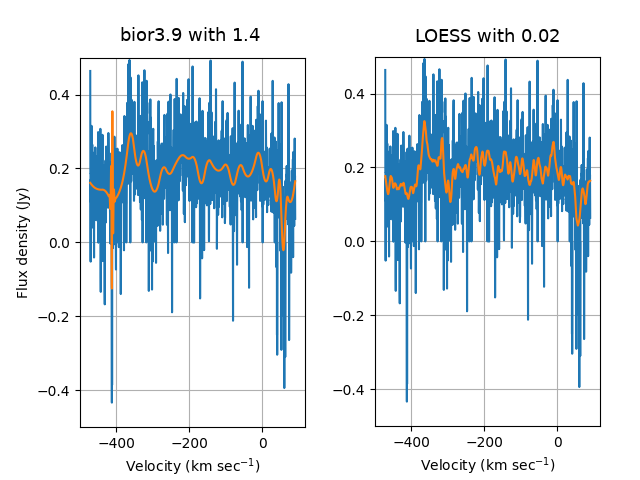
\includegraphics[width=\textwidth]{images/created/method-compare.png}
\caption{Panstarrs C/2017 T2 datu kreisās cirkulārās polarizācijas metožu salīzinājums}
\label{fig:loess}
\end{figure}


\section{ACU žurnalēšanas faili}

Bakalaura darba ietvaros, tika izveidotas vairākas kļūdu kontroles sistēmas, viena no tām - ACU žurnalēšanas failu pārbaudes. ACU jeb Antenna Control Unit ir sistēma, kura atrodas uz Fieldsystem aparatūras \cite{fieldsystem}, kas nodrošina radioteleskopa pozicionēšanu pret novērojuma objektu un informāciju par vēlamo un faktisko teleskopa pozīciju (elevācijas un azimuta vērtības) apraksta žurnalēšanas failos jeb ACU log failos. Šāda veida dokumentēšana nodrošina iespēju zināt precīzu antenu stāvokli konkrētos laikos, līdz ar to, lai pārbaudītu datu integritāti, ACU log failu informācija tika salīdzināta ar novērojumu log failiem.




\begin{figure}[h!]
\centering
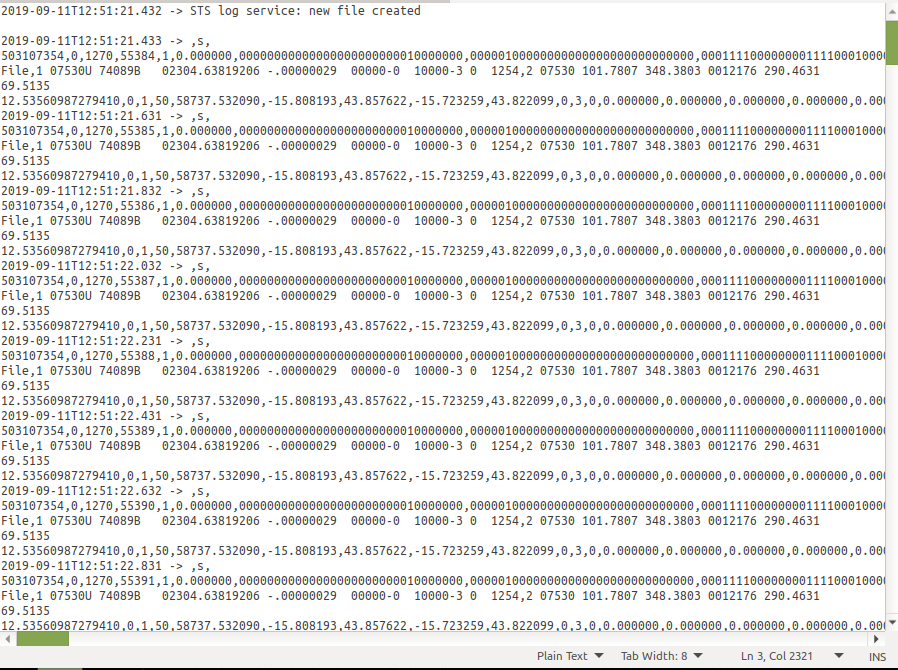
\includegraphics[width=\textwidth]{images/created/acu-img.png}
\caption{ACU sistēmas žurnalēšanas faila piemērs}
\label{fig:acu-example}
\end{figure}

Plašais informācijas daudzums, kurš tiek ierakstīts ACU žurnalēšanas failos arī apgrūtina vieglu informācijas nolasīšanu. Žurnalēšanas faila katra rinda sākās ar ierakstīšanas laiku, kuram seko informācija par ierakstu. Informācija ierakstīta \textit{CSV} stilā, taču informācijai ir ap 200 kolonnām. Ne visas kolonnu vērtības ir vienā formātā, kas vēl vairāk apgrūtina datu nolasīšanu. Vienā žurnalēšanas failā pēc noklusējuma ierakstītas ap 10 000 rindām, kur katrā rindā ir vidēji 2300 simboliem, atkarībā no rindas tipa. Attēlā \ref{fig:acu-example} atspoguļots ACU žurnalēšanas faila sākums no 2019.gada 11. septembra ierakstīšanas sesijām.

Salīdzināšanas sākumā tiek nolasītas visas laika vērtības no novērojuma log faila, kā arī atbilstošās azimuta un elevācijas vērtības šajā laikā. Ņemot vērā, ka ACU logu intervāls starp ierakstiem ir mazāks par 200 milisekundēm, bet novērojumu log failos ierakstu intervāls ir ap 20 sekundēm, identiskus laikus nevar atrast, novērojumu log failu neprecizitātes dēļ. Šī iemesla dēļ tiek izmantots viens no ACU log ierakstiem konkrētā sekundē.  


No ACU logiem tiek nolasīta tekošā pozīcija saskaņā ar enkoderi un uzdotā pozīcija. Nolasītās vērtības tiek salīdzinātas ar novērojumu log failu azimuta un elevācijas vērtībām un tiek izvadīti grafiki salīdzināšanai, kā arī tiek aprēķinātas atšķirības starp vērtībām, izvadot attiecīgus grafikus. Visām šīm vērtībām vajadzētu būt aptuveni vienādām, līdz ar to, ja ir instances kurās vērtības atšķiras, novērojumu skanos ir bojājumi. Grafiki palīdz atrast kļūdas un dod iespēju informēt inženierus par laikiem, kuros anomālijas ir atrastas, lai novērstu problēmas nākotnē.

Grafika piemērs attēlots \ref{fig:acu-example-plot} attēlā, kur aprēķināts OH māzera g126p715 0p822 žurnalēšanas failā ierakstīto elevācijas un azimuta vērtību salīdzinājums ar ACU žurnalēšanas failā ierakstītajām. Rezultāts attēlots, kā sekunžu atšķirība starp abu žurnalēšanas failu  elevācijas vērtībām, konkrētajos laikos. Kā \textit{el\_deltaPlst} un \textit{az\_deltaPlst} tiek attēlots elevācijas un azimuta tekošā pozīcija saskaņā ar enkoderi, bet ar \textit{az\_deltaPsoll} un \textit{el\_deltaPsoll} - uzdotā pozīcija.


\begin{figure}[H]
\centering
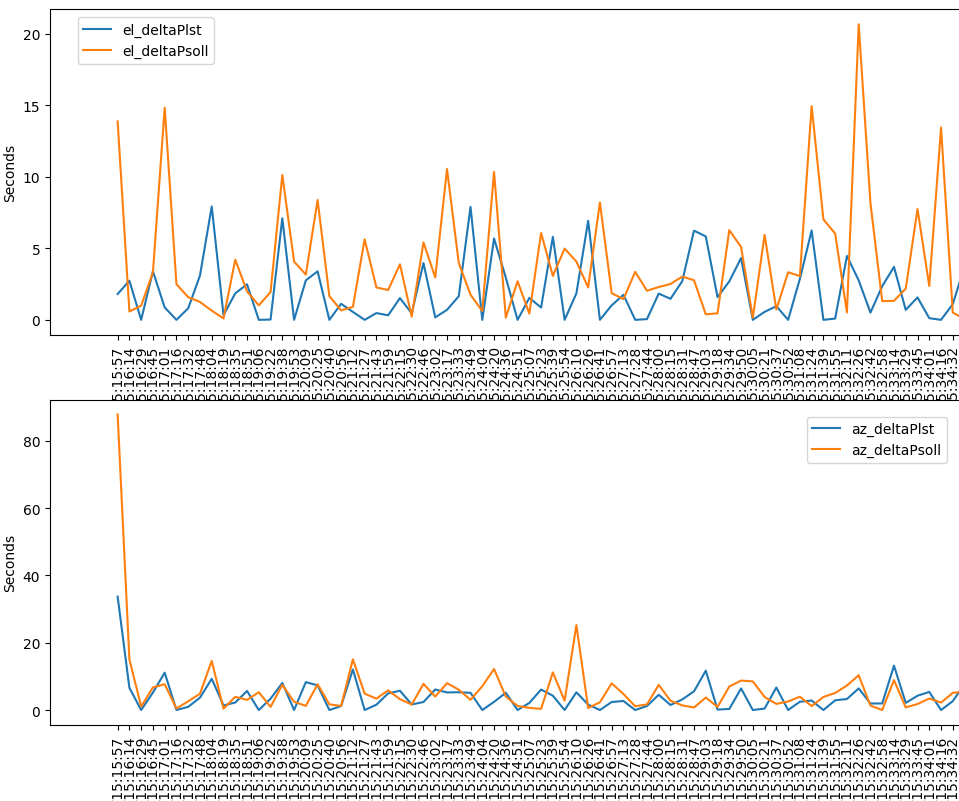
\includegraphics[width=\textwidth]{images/created/ACU-example.png}
\caption{ACU žurnalēšanas faila salīdzinājuma rezultāts}
\label{fig:acu-example-plot}
\end{figure}
%un citi apskatītie
%\subsection{Kalibrācijas integrācija ACOR sistēmā}
%Aprakstīt nedaudz kas tā ir un kas tika izdarīts prakses laikā sakarā ar šo. Aprakstīt kāpēc ir problēmas ar to risinājumu un kā varētu risināt. Ja sanāks laika tad arī risinājumu.

\section{Nākotnes plāni un datu apstrādes tālākie soļi}




Vāju radioastronomisku signālu apstrāde ir sarežģīts process, līdz ar to ir dažādas pieejas katrai problēmai. To efektivitāti iespējams pārbaudīt tikai ar realizāciju, taču visas metodes nebija iespējams apskatīt Bakalaura darba ietvaros, līdz ar to, nodaļā aprakstīti potenciālie uzlabojumi un apstrādes tālākie soļi.

%KLT
Potenciāls uzlabojums apstrādes rezultātos ir iespējams jau datu nolasīšanas brīdī, kur Furjē transformācijas procesu var aizvietot ar Karhunen—Loève Transform \cite{KLT}. Izmantojot minēto apstrādes metodi, tehniski ir iespējams detektēt ļoti vājus signālus attiecībā pret troksni, jo metode izmanto matricu ar nejauši ģenerētiem skaitļiem un veic kompleksus lineārās algebras aprēķinus, lai iegūtu vislabākos koeficientus, kurus izmanto, lai iegūtu spektra frekvenču amplitūdu vērtības. Lai gan vēl nav izpētīts metodes pielietojuma iespējamība radioastronomiskajiem datiem, iespējams, ka, izmantojot minēto metodi, vāju objektu detektēšana būtu efektīvāka.

%Stokes parametri
Lai nodrošinātu datu integritāti un iegūtu papildus informāciju par novērojamo objektu, tika apskatīti arī Stoka \cite{stokes-theory} parametri - vērtību kopa, kas apraksta polarizācijas radiācijas stāvokli. Balstoties uz rakstu par Nançay radioastronomijas observatorijas iegūtajiem rezultātiem 2007.-2009. gada intervālā \cite{nancay}, kurā tika aprakstīta informācija par laika periodā novērotajām maiņzvaigznēm, bija iespējams salīdzināt šos rezultātus ar Bakalaura darba laikā apskatītā objekta rezultātiem. Bakalaura darba ietvaros tika izpētīts \textit{The Measurement of Polarization in Radio Astronomy} \cite{stokes} raksts, lai iegūtu formulas cirkulārās polarizācijas Stokes parametru aprēķinam, taču iegūtos rezultātus nevarēja uzskatīt par pārliecinošiem, līdz ar to tie netiek aprakstīti Bakalaura darba ietvaros.
%\begin{equation}
%I= \langle E_R^2 \rangle + \langle E_L^2 \rangle \tag{2.2.5.1}\label{eq:2.2.5.1}
%\end{equation}
%\begin{equation}
%Q = 2 \langle Re(E_R E_L^*) \rangle = 2 \langle E_R E_L \cos{\delta_{RL}} \rangle \tag{2.2.5.3}\label{eq:2.2.5.3}
%\end{equation}
%\begin{equation}
%U = 2 \langle Im(E_R E_L^*) \rangle = 2 \langle E_R E_L \sin{\delta_{RL}} \rangle \tag{2.2.5.4}\label{eq:2.2.5.4}
%\end{equation}
%\begin{equation}
%V= \langle E_R^2 \rangle - \langle E_L^2 \rangle \tag{2.2.5.5}\label{eq:2.2.5.5} 
%\end{equation}

%\textbf{paskaidrojums un kur/kāpēc tiek izmantots}
%kur: 
%\begin{tabbing}
%\phantom{\hspace{10mm}}\= \kill
%$I$\>                   =$I$\\
%$Q$\>                   = $Q$\\
%$U$\>                   = $U$\\
%$V$\>                   = $V$\\
%$E_R^2$\>               = $E_R^2$\\
%$E_L^2$\>               = $E_L^2$\\
%$\delta_{RL}$\>         = $\delta_{RL}$\\

%\end{tabbing}
%Rakstā tika apskatītas kopā 70 zvaigznes, taču bakalaura darba ietvaros, tika apskatīta tikai informācija par RLMI maiņzvaigni, jo minētais objekts tika novērots, kā komētu kalibrators. 

Stoka parametri sniedz informāciju arī par objekta magnētiskā lauka stāvokli, līdz ar to, papildus izmantojot iegūtos datus kopā ar optiskiem novērojumiem, iespējams veidot OH māzeru spilgtuma modeļus, kā arī veikt objekta monitoringu. Lai gan Bakalaura darbā sadarbība nav realizēta, nākotnē ir potenciāls veidot minēto sadarbību ar kādu optisko novērojumu observatoriju, piemēram, Baldones observatoriju.

Komētu novērojumiem arī ir potenciāls izmantot \textit{Very-Long-Baseline Interferometry} metodes, kur signāls no viena astronomiska objekta tiek novērots ar vairākiem radioteleskopiem vienlaicīgi. Vairāku neatkarīgu staciju novērojumu veikšana vienlaicīgi samazina iespēju veikt inženiertehniskās kļūdas, kā arī sniedz daudz vairāk datu. Lai gan VSRC ir iesaistīts VLBI novērojumos, novērojumu veikšana ir process, kas prasa daudzu staciju sadarbību, kā arī jaunu sistēmu ieviešanu, līdz ar to metodikas ieviešana prasītu ilgu laiku, taču varētu novest pie daudz labākiem rezultātiem.

